\documentclass[10pt,twocolumn,letterpaper]{article}

\usepackage{cvpr}
\usepackage{amsmath}
\usepackage{amssymb}
\usepackage{caption}
\usepackage{booktabs}
\usepackage{graphicx}

\definecolor{cvprblue}{rgb}{0,0,0}
\usepackage[pagebackref,breaklinks,colorlinks,allcolors=cvprblue]{hyperref}

\title{Autoencoding Gaussian Splats in 2D}

\author{Rok Mokotar\thanks{Both authors are students at Ludwig Maximilian University of Munich, Geschwister-Scholl-Platz 1, 80539 Munich, Germany. They contributed equally to this work in all aspects, including conceptualization, research, and writing. The order of authorship was determined randomly and does not reflect any difference in their contributions.}\\
LMU Munich\\
{\tt\small Rok.Mokotar@campus.lmu.de}
\and
Federico Bernardo Harjes Ruiloba\footnotemark[1]\\
LMU Munich\\
{\tt\small f.harjes@campus.lmu.de}
}

\begin{document}
\maketitle
\begin{abstract}
TODO - at the end :D
\end{abstract}
\section{Introduction}
\label{sec:introduction}

Recent advances in neural rendering and generative modeling have demonstrated the effectiveness of 	Gaussian splatting for representing images and 3D scenes. In this work, we explore the novel task of 	autoencoding for Gaussian splats, where we leverage autoencoders (AEs) to learn compact representations of images modeled as 2D Gaussian splats. Our primary objectives are twofold: \textit{(1)} to construct and train an autoencoder for Gaussian splat representations of images and \textit{(2)} to compare its performance against a standard autoencoder trained directly on raw image data. 

The importance of this problem arises from the growing need for efficient and flexible representations of visual data. Gaussian splats offer a structured and parametric alternative to pixel-based representations, encapsulating key image features such as position, scale, rotation, opacity, and color in a compact form. This representation aligns well with modern neural rendering techniques and has the potential to enhance interpretability, adaptability, and compression efficiency in learned visual representations.

We adopt Gaussian splats and autoencoders for this task due to their complementary strengths. Gaussian splatting has proven to be a powerful representation technique for reconstructing visual data with high fidelity while being inherently adaptable to multi-resolution settings. Autoencoders, on the other hand, provide a well-established framework for extracting meaningful latent representations and reducing data dimensionality in an unsupervised manner. By combining these approaches, we aim to investigate whether autoencoding in the Gaussian splat space can yield benefits in terms of compression efficiency, reconstruction quality, and feature disentanglement compared to standard pixel-based autoencoding.

A key focus of this work is on the compression capabilities of Gaussian splats. Unlike traditional pixel-based approaches, where compression often relies on feature extraction in a high-dimensional space, Gaussian splats inherently provide a more structured, lower-dimensional representation of images. This opens up opportunities for novel encoding strategies that take advantage of the underlying parametric nature of the splat representation.

Our contributions in this study include:
\begin{itemize}
    \item The creation of a dataset consisting of trained Gaussian splats derived from CIFAR-10 images, enabling further research on learned splat representations.
    \item The design and implementation of an autoencoder specifically tailored for Gaussian splats, exploring different architectural choices and their impact on reconstruction quality.
    \item A comparative analysis of Gaussian splat-based autoencoding against conventional pixel-based autoencoding to evaluate reconstruction performance and compression efficacy.
\end{itemize}

By addressing these objectives, we aim to provide insights into the potential of Gaussian splats as a learned visual representation and contribute to the broader research on neural compression and generative modeling.

The remainder of this report is structured as follows: Section \ref{sec:background} provides essential background on Gaussian splatting and autoencoders. Section \ref{sec:methodology} details our dataset, splatting process, autoencoder design, and experimental setup. Section \ref{sec:results} presents our findings on different splatting techniques, autoencoder architectures, and various evaluation approaches. Section \ref{sec:discussion} interprets the results, highlighting key insights, limitations, and future directions. Finally, Section \ref{sec:conclusion} summarizes our contributions.  


\section{Background}
\label{sec:background}

\subsection{Gaussian Splats}
\label{bg-gs}
Recently, scene representation and novel-view synthesis techniques making use of machine learning methods have gained attention. One of the most popular frameworks in this category are Neural Radiance Fields (NeRFs) $\cite{}{}$, able to produce high quality implicit representations of scenes. Typically, NeRFs do this by optimizing a deep neural network using a volumetric continuous representation of the scene, using thechniques such as volumetric ray marching. In spite of various improvements to increase the efficiency of this framework $\cite{}{}$, achieving high visual quality through NeRFs remains computationally expensive due to the training cost of the neural network, in addition to a high rendering cost. To address these issues, the Gaussian Splatting (GS) framework was proposed.

Through Gaussian Splatting, instead of learning a continuous implicit representation of a scene, scenes are explicitly represented through a set of points using a large number of Gaussian primitives. The Gaussian ellipsoids constituting a scene have a set of learnable parameters controlling properties of the reconstruction, such as position, opacity, anisotropic covariance, and spherical harmonic (SH) coefficients. In addition to providing a high reconstruction quality, Gaussian Splatting provides much faster rendering, being able to produce novel-views in real time. GS achieves this by using rasterization-based rendering, which, in contrast to the rendering used by NeRFs, does not require sampling points.

Although GS was originally formulated for the reconstruction of 3D-scenes, and is often studied in that domain, this work considers 2D GS. Considering 2D GS alleviates some of the challenges involved in the process of auto-encoding Gaussian Splats.

\subsection{Auto-Encoders}


\label{bg-ae}
\section{Methodology}
\label{sec:methodology}

\subsection{Dataset}
In our study, we used the CIFAR-10 dataset \cite{krizhevsky2009learningml}, a widely recognized benchmark for machine learning and computer vision algorithms. It consists of $60,000$ color images of size $32 \times 32$ pixels, categorized into 10 evenly distributed classes. The dataset is originally divided into $50,000$ training images and $10,000$ test images.

As mentioned earlier, our goal was to construct a dataset of trained Gaussian Splats, where each Gaussian encapsulates local image features based on the CIFAR-10 dataset. We generated this dataset by mapping each image to a set of five Splat parameters: position (mean), scale, rotation (quaternion), opacity, and color. Each parameter is represented as a $1024 \times N$ matrix, capturing the spatial, color, and intensity distributions across the image. The dataset is implemented as a \texttt{PyTorch} dataset \cite{paszke2019pytorchai}, partitioned into training, validation, and test sets using a $4 : 1 : 1$ split.

\subsection{Gaussian Splatting}
To construct a dataset suitable for training an AE for Gaussian Splats, it was essential to first establish an effective method for generating high-quality Gaussian representations of images.

\paragraph{Gaussian representation and optimization.}
We employed the \texttt{gSplat} library \cite{ye2024gSplatao} to convert images into Gaussian Splats. The primary objective was to optimize the placement and parameters of the Gaussians to achieve the most accurate rasterization possible. Various configurations and hyperparameters were explored to assess their impact on the accuracy of the reconstructed images. The implementation was modular, allowing for flexible adjustments and systematic evaluation of different settings. 

A key aspect of our methodology was the optimization process, where we implemented and tested several parameter learning strategies, including:

\begin{itemize}
    \item training iterations and learning rate: adjusting the number of optimization steps and the step size for parameter updates,
    \item loss functions: evaluating different combinations of loss functions (L1, L2, SSIM) to determine their impact on image reconstruction quality,
    \item regularization strategies: applying constraints on scales and opacities to prevent degenerate solutions,
    \item optimization techniques: experimenting with group optimization and adaptive gradient strategies such as selective Adam and sparse gradient methods,
    \item scheduling and optimization strategies: implementing various learning rate schedulers and optimization algorithms to improve convergence.
\end{itemize}

\paragraph{Extended functionality and dataset variants.}
To enhance the flexibility of Gaussian Splatting, we incorporated additional features, including:

\begin{itemize}
    \item selective learning of Splat parameters: allowing control over which Gaussian parameters are optimized during training,
    \item support for 2D and 3D rasterization: implementing both standard 2D rasterization and extending compatibility with custom 3D rasterization techniques \cite{kerbl20233dgs},
    \item bilateral guided radiance support: integrating methods for improved radiance-based rendering \cite{wang2024bilateralgr}.
\end{itemize}

Furthermore, we explored different initialization strategies to generate diverse dataset variants, implementing three approaches:

\begin{itemize}
    \item random initialization: assigning Gaussian parameters randomly within predefined bounds,
    \item grid-based initialization: placing Gaussians on a structured grid for uniform coverage,
    \item KNN-based initialization: distributing Gaussians based on a nearest-neighbor approach to better approximate image structures.
\end{itemize}

These variations allowed us to construct multiple datasets tailored to different experimental conditions, enabling a comprehensive evaluation of autoencoding techniques for Gaussian Splats.

\paragraph{Autoencoder architectures.}
After generating Gaussian Splats, we implemented three distinct AE architectures: a deep AE, a convolutional AE, and a ResNet-based AE. Each model was designed as an implementation of our abstract AE module in \texttt{PyTorch} \cite{paszke2019pytorchai}, ensuring architectural flexibility and a standardized training pipeline.

The deep AE processes an input vector of dimension $23552$, encoding it into an $N$-dimensional latent space through four fully connected feed-forward layers. The decoder is a mirrored version of the encoder, with a final $\tanh$ activation to constrain outputs within the original value range.

The convolutional AE takes as input a $32 \times 32 \times N$ matrix representation, where $N$ denotes the number of channels. The encoder consists of three sequential convolutional and max-pooling layers. The decoder, built using three transposed convolutional layers, reconstructs the original input with a $\tanh$ activation.

The ResNet-based AE follows the architecture of ResNet-18 \cite{he2015deeprl}, with modifications inspired by the convolutional AE. The residual connections enhance gradient flow, improving learning stability and convergence.

\paragraph{Experimental setup and training.}
To evaluate the models, we conducted multiple experiments tailored to different representations of Gaussian Splats:

\begin{itemize}
\item vector-based encoding: the deep AE was tested on a flattened representation, combining all Gaussian parameters into a single vector to assess the importance of spatial information,
\item full-image encoding: the convolutional and ResNet-based models were trained on a transformed image representation where all 23 parameter channels were combined and learned simultaneously,
\item single-channel encoding: an alternative approach involved training models on individual parameter channels, treating them as separate grayscale images to examine per-parameter learning efficiency,
\item independent parameter models: a final experiment trained a distinct AE for each Splatting parameter, allowing for independent optimization but at the cost of increased complexity.
\end{itemize}

\paragraph{Hyperparameter optimization.}
A crucial part of our methodology was optimizing hyperparameters to enhance performance. The training pipeline systematically explored the following factors:

\begin{itemize}
\item latent dimension: determining the optimal size of the compressed representation for effective reconstruction.
\item learning rate and weight decay: evaluating their impact on stability and convergence using the Adam optimizer.
\item number of epochs and gradient clipping: preventing instability in training dynamics,
\item initialization strategies: comparing standard and Xavier weight initialization techniques,
\item regularization techniques: assessing dropout and batch normalization effects on generalization,
\item learning rate scheduling: experimenting with different schedulers to adapt learning dynamics.
\end{itemize}

\section{Results}
\label{sec:results}

\subsection{Gaussian Splatting}
\paragraph{Hyperparameter tuning.} To achieve our first goal, producing a dataset of Gaussian Splats that represent CIFAR-10 images as accurately as possible, we performed a thorough hyperparameter optimization using the \texttt{Optuna} library. 

As expected, the number of Gaussian primitives used was the most influencing factor on reconstruction quality. We tested using $256$, $1024$ and $4096$ Gaussians, and found $1024$ to be a good compromise between reconstruction quality and training efficiency. More interestingly, the opacity regularization factor had a particularly large impact on the optimization result. The initial scale of the Splats also played an important role. More details about the hyperparameter tuning process can be found in the Appendix.

\paragraph{Training and dataset generation.}
In addition to finding optimal hyperparameters for reconstructing the CIFAR-10 images with high fidelity, we found that among the three initialization strategies — random, grid-based and KNN-based — the grid and KNN strategies clearly yielded better reconstructions. For this reason, we decided to generate two datasets of trained Splats for the $60,000$ CIFAR-10 images corresponding to these different initialization strategies.

The rasterized images corresponding to the trained Splats resemble the original images accurately for both grid- and KNN-based initializations, as shown in Fig. \ref{fig:Splat-reconstructions}. While the KNN-based Splats achieved significantly lower losses during training, the grid-based images seem to be visually closer to the original images in most cases, as can be noticed in the images corresponding to the automobile, deer, ship and truck classes. In some instances, the KNN-based Splats achieved a higher accuracy on local details, such as for the frog's eye or the horse's head.

The two generated Gaussian Splat datasets were implemented as \texttt{PyTorch} datasets using a 4 : 1 : 1 split for training, validation, and test sets. The full datasets have a size of approximately 5 GB.

\begin{figure*}
    \centering    \includegraphics[width=1\linewidth]{fig/Splat_reconstruction_comparison.pdf}
    \caption{\textbf{Gaussian Splat Reconstruction of the CIFAR-10 Classes.} Example reconstructions for one of each CIFAR-10 classes. The top row shows the original image, while the middle and lower rows show the Gaussian Splat reconstructions using the grid- and KNN-initializations respectively.}
    \label{fig:Splat-reconstructions}
\end{figure*}

\subsection{Auto-encoding of 2D Splats}
\paragraph{Hyperparameter Tuning.} 
Similarly to the case of the Gaussian Splat dataset generation, we performed a detailed hyperparamter tuning process to find the optimal configuration for each AE variant through \texttt{Optuna}. Interestingly, we found the most critical hyperparameter to be the rate of weight decay, independent of the model architecture and Splat encoding used. Furthermore, we found the random initialization to work better than a Xavier uniform initialization. More details on the results of the hyperparameter tuning for different architectures can be found in the Appendix.

\paragraph{Model comparison.} 
Of the three model architectures that we trained on the whole Splat dataset, the best results were achieved by our convolutional AE. This model was not only able to outperform the simpler deep AE, but also the more sophisticated ResNet-18 AE for all Splat encoding variants. Among the four Splat encodings we tested, the single-channel encoding, where we treated each parameter channel as a separate grayscale image, produced the best results. A comparison of the loss, calculated as the MSE between the input and output Splat encodings, can be found in Fig. \ref{fig:loss-curves}.

\begin{figure}
    \centering    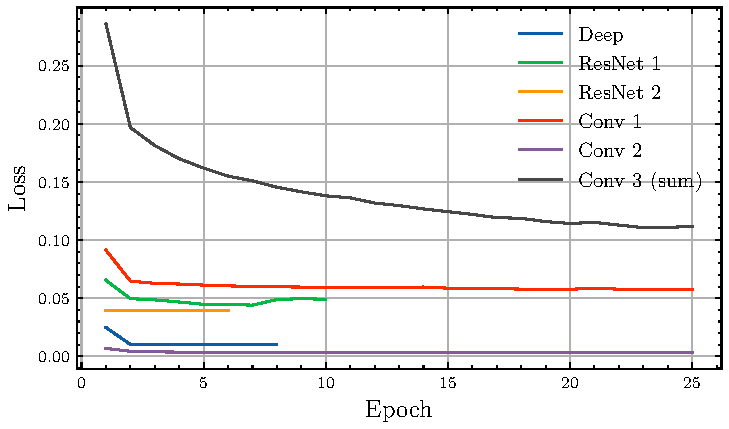
\includegraphics[width=1\linewidth]{fig/loss_curves.pdf}
    \caption{\textbf{Loss Function for Different Model Variants.} The deep model variant used vector encoding, while ResNet 1 and Conv 1 used full-image encoding. Conv 2 and ResNet 2 used single-channel encoding, while Conv 3 trained each parameter independently. In the case of Conv 3, the loss curve shows the sum of individual parameter losses. Some curves are abruptly cut, as the training was stopped early when no improvement was observed.}
    \label{fig:loss-curves}
\end{figure}

\paragraph{Reconstructing the original images.}
Although the MSE between the input and output Splats was extremely close to zero for some models (less than 0.01 in some cases), and the generated input Splats successfully mimic the original images, reconstructing images from AE outputs did not produce entirely satisfactory results. Comparing the renderings created using the outputs of each model, we found that, again, the convolutional model using a single-channel encoding produced the best results. The images reconstructed using the outputs of this model can be found in Fig. \ref{fig:ae-reconstructions}, below the original images from the CIFAR-10 dataset. For comparison, the third row of this figure corresponds to the output of our implementation of a ResNet-18 AE which was trained on raw images instead of Gaussian Splats.

\begin{figure*}
    \centering    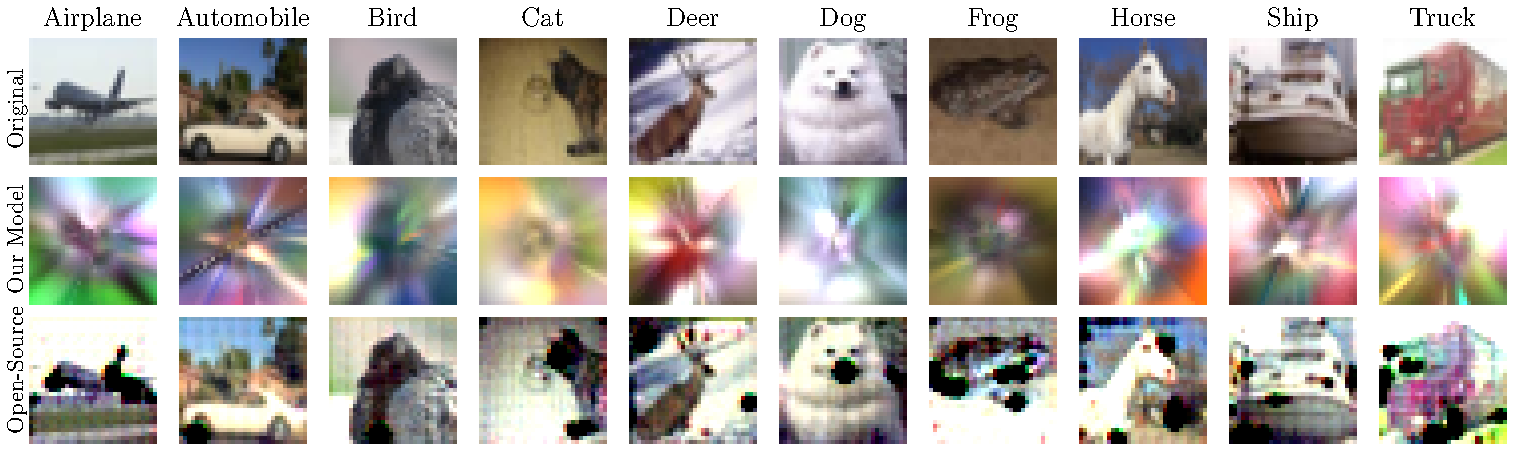
\includegraphics[width=1\linewidth]{fig/reconstruction_comparison.pdf}
    \caption{\textbf{Reconstruction of Autoencoded Images and Gaussian Splats.} The first row on this figure shows 10 random CIFAR-10 images. The second row shows the reconstruction of the CIFAR-10 Splats we generated corresponding to these images, after passing them through our convolutional AE. For comparison, the third row shows the reconstruction of the raw images on the first raw after passing them through our implementation of a ResNet-18 AE.}
    \label{fig:ae-reconstructions}
\end{figure*}

As the convolutional AE with single-channel encoding produced the closest results to the original Splats, we tested training two variants of this model using latent space sizes $4\times4$, corresponding to three Max-Pooling layers, and $8\times8$, corresponding to two Max-Pooling layers. Visually, both model variants produced reconstructions of similar quality, with slightly more accurate colors and structures with a larger latent space, as can be seen in Fig. 9 in the appendix.

\paragraph{Reconstructing individual parameters.}

Considering the lack of a strong visual similarity between the input and output Splats of the AEs despite the low MSE between the tensors representing the Splats, an interesting experiment is visualizing the tensor corresponding to each of the parameters of both input and output Splats. To do this, we visualized the $1024 \times 3$-dimensional parameters as colored images and the $1024$-dimensional parameters as grayscale images. In the case of the quaternions specifying the rotations of the Splats, which have the shape $1024\times4$, we converted them into a three-dimensional rotation matrix, plotted as a colored image. The resulting plots can be found in Fig. \ref{fig:individual-params}.

\begin{figure}
    \centering    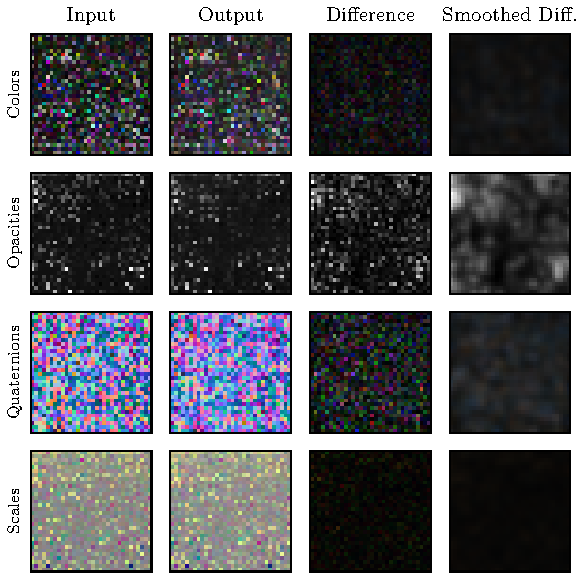
\includegraphics[width=0.97\linewidth]{fig/parameters_individual_viz.pdf}
    \caption{\textbf{Visualization of Individual Parameters of the Input and Output Splats of our Convolutional AE.} Comparison of the tensors corresponding to the individual parameters (colors, opacities, quaternions and scales) of the generated Splats (input) against the same parameters of the autoencoded Splat (output).}
    \label{fig:individual-params}
\end{figure}

This figure reveals that the AEs produced highly similar matrices for every parameter, noticeably almost identical in the case of the colors and scales parameters. This is a particularly interesting result, as it shows that the latent space could represent the most relevant features of the Splats with enough accuracy to reconstruct the parameters with a high fidelity. Furthermore, the latent space of the model was particularly small at a shape of $4\times4$.

\section{Discussion}
\label{sec:discussion}

As mentioned previously, one of the primary objectives of this study was to perform a comparative analysis between our Gaussian splat-based ResNet autoencoder and a more conventional pixel-based ResNet autoencoder. Both approaches, utilizing the same model architecture, were evaluated in terms of compression efficiency and reconstruction performance.

For our model, we trained a ResNet architecture on five separate models, each corresponding to a distinct Gaussian splat parameter, based on our newly created CIFAR-10 dataset of Gaussian splats. In contrast, for the conventional approach, we employed the ResNet-18 model implementation\footnote{\url{https://github.com/eleannavali/resnet-18-autoencoder}} and trained it on the original CIFAR-10 dataset.

Figure \ref{TODO} illustrates the comparison between the two approaches using random test images from each class. The results indicate that our Gaussian splat-based model struggles to reconstruct images effectively, primarily capturing certain relationships related to rotations and colors while failing to preserve finer details and structures. Quantitative analysis, such as the Structural Similarity Index (SSIM), supports this observation, with the SSIM difference between the original and our model being TODO, while the difference between the original and the conventional model is TODO.

Moreover, when comparing the compression ratios between both approaches, the conventional method remains more efficient, achieving a compression ratio of TODO, whereas our model achieves a compression ratio of TODO. This suggests that our approach not only fails to maintain high reconstruction accuracy but also results in inefficient compression, in some cases even increasing the image size. If the compression ratio exceeds 1, further investigation is required to determine whether this is an inherent limitation of our method or a fundamental trade-off associated with representing images using Gaussian splats.

\subsection{Future Work}

Finally, we have identified several potential areas for future research and applications where this approach could be utilized:

\begin{itemize}
    \item \textbf{Exploring the effect of latent space size on reconstruction error:} It would be valuable to investigate how the reconstruction error sinks as the size of the latent space increases. Understanding this relationship could help optimize the balance between compression efficiency and reconstruction quality.
    
    \item \textbf{Loss function refinement:} An interesting avenue of investigation would be to explore whether the autoencoder should be trained by minimizing the loss based only on the Gaussian splats, or if it would be beneficial to enforce consistency between the rendered splat and the original image. This could potentially improve the reconstruction accuracy or reduce artifacts.
    
    \item \textbf{Implementation of Hierarchical Perceiver (HiP):} Incorporating HiP, as discussed in \cite{carreira2022hierarchicalp}, could be an interesting future work. The hierarchical nature of HiP may provide better structure to the encoding process, enhancing performance on Gaussian splats.
    
    \item \textbf{Latent space classification:} Exploring the possibility of using the latent space for downstream tasks, such as classification, could open up new applications for Gaussian splat-based representations.
    
    \item \textbf{Generative modeling on the latent space:} Building a generative model (e.g., Generative Adversarial Networks or Stable Diffusion) on top of the latent space could allow us to generate new images or 3D scenes from the compressed representations, facilitating content creation or data augmentation tasks.
    
    \item \textbf{Gaussian splat generation:} Developing a model capable of generating new Gaussian splats (e.g., a Variational Autoencoder) would be an intriguing direction. This could lead to more sophisticated image synthesis techniques, allowing us to generate realistic images directly from the splat parameters.
    
    \item \textbf{Masked Autoencoders (MAE) for smaller images:} Finally, investigating the application of MAE on smaller images could help determine if this approach could provide more efficient representations and faster processing times, especially in cases where the dataset is constrained in size.
\end{itemize}

\section{Conclusion}
\label{sec:conclusion}
{
    \small
    \bibliographystyle{ieeenat_fullname}
    \bibliography{main}
}

\end{document}
